\section{Chemical Equations} \index{Chemical equations} \index{Equations} \index{Chemical reactions}

\begin{multicols}{2}


%\section*{}


\subsection{Balancing Reactions}

\begin{center}
%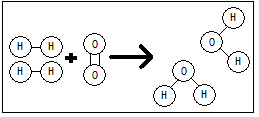
\includegraphics[width=0.4\textwidth]{./img/balancing-reactions.png}
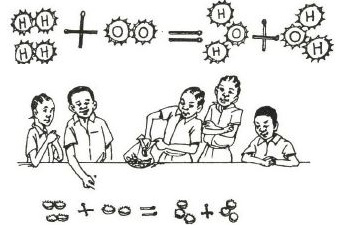
\includegraphics[width=0.4\textwidth]{./img/source/chem-equations.jpg}
\end{center}

\begin{description*}
%\item[Subtopic:]{}
\item[Materials:]{Bottle caps, matches}
%\item[Setup:]{}
\item[Procedure:]{Use bottle caps and matches to construct the reactants and products of a chemical reaction (e.g. $2\mathrm{H}_2 + \mathrm{O}_2 \longrightarrow 2\mathrm{H}_2\mathrm{O}$). }
%\item[Hazards:]{}
%\item[Questions:]{}
\item[Observations:]{It can be seen visually how atoms rearrange to form new molecules.}
%\item[Theory:]{}
%\item[Applications:]{}
%\item[Notes:]{}
\end{description*}

\subsection{Combination Reactions}

%\begin{center}
%\includegraphics[width=0.4\textwidth]{./img/.jpg}
%\end{center}

\begin{description*}
%\item[Subtopic:]{}
\item[Materials:]{Sulphur, steel wool, \nameref{sec:heatsources}, spoon, bar magnet, bottles}
%\item[Setup:]{}
\item[Procedure:]{Grind the steel wool to get fine particles. Place a small amount in a bottle and add an equal amount of sulphur powder. Hold a magnet above the mixture and observe. Then heat a small amount of iron filings with twice as much sulphur until the sluphur powder is gone. Again try to separate the mixture with a bar magnet. Finally heat a mixture of the two for an extended time and try to separate with a magnet.}
\item[Hazards:]{This reaction produces sulphur dioxide, a poisonous gas. Perform outside or in a well-ventilated room.}
%\item[Questions:]{}
%\item[Observations:]{}
\item[Theory:]{Combination is the kind of chemical reaction where two elements come
together to form a single compound. The mixture can easily be separated before heating because the iron is magnetic while the sulphur is not. When heated, the iron and sulphur combine to form iron (II) sulphide. Because the two are bound together, they cannot be separated by physical means. When heated for a long time, however, the sulphur escapes as sulphur dioxide, leaving behind iron oxide (a metal) which can be picked up with a magnet.}
%\item[Applications:]{}
%\item[Notes:]{}
\end{description*}

\subsection{Precipitation Reactions}

%\begin{center}
%\includegraphics[width=0.4\textwidth]{./img/.jpg}
%\end{center}

\begin{description*}
%\item[Subtopic:]{}
\item[Materials:]{Copper sulphate, soda ash (sodium carbonate), containers, funnel, cloth}
\item[Setup:]{Make solutions of copper sulphate and sodium carbonate by mixing a spoonful in about 500 mL of water (in separate containers).}
\item[Procedure:]{In a container, combine a small amount of each solution and filter using a cloth or toilet paper.}
%\item[Hazards:]{}
%\item[Questions:]{}
%\item[Observations:]{}
\item[Theory:]{A precipitate reaction is the formation of an insoluble salt by mixing solutions
which contain its two components. When copper sulphate solution is mixed with sodium carbonate a blue precipitate (calcium carbonate) will form. This reaction is useful for
preparing insoluble salts. The chemical reaction is:\\
\ce{CuSO4_{(aq)} + Na2CO3_{(aq)} -> CuCO3_{(s)} + Na2SO4_{(aq)}} }
%\[ \mathrm{CuSO}_{4(aq)} + \mathrm{Na}_2\mathrm{CO}_{3(aq)} \longrightarrow \mathrm{CuCO}_{3(s)} + \mathrm{Na}_2\mathrm{SO}_{4(aq)} \]}
%\item[Applications:]{}
%\item[Notes:]{}
\end{description*}

\subsection{Decomposition Reactions}

%\begin{center}
%\includegraphics[width=0.4\textwidth]{./img/.jpg}
%\end{center}

\begin{description*}
%\item[Subtopic:]{}
\item[Materials:]{Copper carbonate, citric acid, spoon, \nameref{sec:heatsources}}
\item[Setup:]{Dry the copper carbonate from the precipitation reaction by leaving in an open container.}
\item[Procedure:]{Heat a small sample of copper carbonate in a spoon until only a black residue remains. Add a small amount of citric acid and heat again until only a black residue remains.}
%\item[Hazards:]{}
%\item[Questions:]{}
%\item[Observations:]{}
\item[Theory:]{Thermal decomposition is when a compound breaks down when heated. When copper carbonate is heated, it decomposes to release carbon dioxide. The black reside can be found by subtracting carbon dioxide from the formula for copper carbonate:
\begin{center}
\ce{CuCO3_{(s)} -> CO2_{(g)} + CuO_{(s)}}
%\[ \mathrm{Cu}\mathrm{CO}_{3(s)} \longrightarrow \mathrm{CO}_2 + \mathrm{CuO}_{(s)} \]
\end{center}
When citric acid is heated, it decomposes twice. First, bubbles of carbon
dioxide are released and then, citric acid further decomposes to release water
vapor. The black residue at the end of the experiment is solid carbon.}
%\item[Applications:]{}
%\item[Notes:]{}
\end{description*}

%==================================================================================================%


\end{multicols}

\pagebreak